%\documentclass[11pt, twocolumn]{enscStyle}
\documentclass[12pt]{enscStyle}

\renewcommand{\baselinestretch}{1.1}

%#######################################
% 	Title page info
%#######################################

\title{Shockingly Fun}

\prof{Professor M. Moallem}

\coursecode{ENSC 384}

\date{\today}

\author{
	Dan Hendry (30113878) \\
	Brian Hook (200046894) \\ 
	John Jamel (301080425) \\
	Reza Khatami (301075855) 
}

\begin{document}

%\pagenumbering{roman}

\maketitle

%%%%%%%%%%%%%%%%%%%%%%%%%
% Tables
%%%%%%%%%%%%%%%%%%%%%%%%%


%\tableofcontents
%\addcontentsline{toc}{chapter}{\hspace{13pt}Contents}

%\cleardoublepage

%\pagenumbering{arabic}

%#######################################
% 	Main Section
%#######################################

% Intro
% 	- John
\chapter{Introduction}

This report describes an implementation of the classic two player game PONG using an HCS12 microprocessor and a serial controlled, OLED (organic light emitting diode) screen.
Chapter \ref{ch:support} describes various functionality required by the project including an overview of the methods used to control the OLED.
A description of the techniques used in communication between the HCS12 and OLED, as well as the method used to create pseudrandom numbers, and an overview of techniques which allow C and assembly code to be used in tandem is also presented.
Chapter \ref{ch:pong} contains details of the PONG program itself, including how the players' paddles and the ball are moved and controlled, and how the LCD (liquid crystal display) is used to display a scores.
Finally, a complete listing of source code is presented in appendix \ref{ch:code}.

\section{Rules and Game Objectives}

The rules of this game are quite simple, and very similar to the original PONG's.
Two players, using buttons, are able to move rectangular \q{paddles} on the OLED screen.
Movement is constrained in the vertical direction, within the bounds of the screen.
A ball bounces between the two paddles.
The ball begins in the center of the screen, and begins moving in a pseudorandomly selected direction, continuing to move in the along the same vector until it reaches either the top or bottom of the screen, which cause it to assume the opposite velocity in the y-direction; or either the left or right side of the screen, which causes the player whose paddle is on the opposite side to the screen to have scored a point.
Either player may reflect the ball, using their paddle, by having the ball come into contact with the paddle, causing the ball to take on a pseudorandom velocity in the opposite x-direction.
The game objective of each player, scoring on their opponent is tracked on the LCD screen on the Dragon12 board.

\section{System Components}

The figure below illustrates the basic configuration of the system used in this project, which is an integrated 'Dragon12' board consisting of an HCS12 microprocessor, with a variety of other hardware.
One of the integrated devices on the Dragon12 is an LCD directly connected to a digital I/O port of the microprocessor.
It consists of two-lines of alphanumeric text and is used to display the current score.
A full color, 320 by 240 pixel OLED external to the Dragon12 board was connected to another one of the microprocessor's digital I/O ports, and communicates with it via RS232 protocol, for the purpose of serving as the game display.

\begin{figure}[htp]
    \centering
    \includegraphics[width=.6\textwidth]{images/SystemDiagram.pdf}
    \caption{System Diagram}
    \label{fig:sysdiag}
\end{figure}

%
%Design and simulation
%	- Dan
%
%Section Oscillator
% Design
%	Find R and C Values
%	Given Frequency
%	Use f = 1/(T1+ T2) from lecture notes
%	R3 & R4 From given circuit diagram
%	Just plug in to equations which were given
% Simulation 
%	Using LT Spice
%	-> Todo
% 
\section{Circuit Design and Operation}

This section examines the amplifier control circuit, specifically the PWM oscillator.

%TODO: discussion of operation

\subsection{Selection of Component Values}

The desired PWM oscillation frequency for the circuit is 300 Hz.
A diagram for the oscillator, taken from the instruction manual for the motor control kit, may be seen in figure 1; component numbers used henceforth refer to this diagram.
As presented during lecture, equations \ref{eq:T1} and \ref{eq:T2} show the two time components of the oscillator output, rise time and fall time.
Given the 300 Hz desired frequency, component values must be found to satisfy equation \ref{eq:desiredF}.
 
\begin{figure}[h]
    \label{fig:oscillatorcapture}
    \centering
    \includegraphics[width=.22\textwidth,bb=0 0 300 419]{images/OscillatorCapture.PNG}
    \caption{Circuit Oscillator Circuit - From Manual}
\end{figure}
 
\begin{equation}
	\label{eq:T1}
	T_1 = {\it R_5}\,C\ln  \left( {\frac {{\it R_3}\,{\it V^+}}{{\it R_4}\, \left( {
\it V^+}-{\it V_{in}} \right) }}+1 \right) 
\end{equation}

\begin{equation}
	\label{eq:T2}
	T_2 = {\it R_5}\,C\ln  \left( {\frac {{\it R_3}\,{\it V^+}}{{\it R_4}\,{\it V_{in}}}
}+1 \right) 
\end{equation}

\begin{equation}
	\label{eq:desiredF}
	300= {\frac {1}{T_1 + T_2}}
\end{equation}

There is a single constraint equation (the frequency) and four component values appearing in the equation which must be chosen.
As such, three component values must be fixed, arbitrarily or based on external constraints, to solve for the last component value which gives a 300 Hz frequency.
%
%More explanaition of the following might be needed
Resistor $R_3$ acts to scale the input voltage and therefore only impacts frequency to the extent that the input voltage does.
Similarly, resistor $R_4$ simply determines the gain of the op-amp, and offsets the output voltage. 
The values for $R_3$ and $R_4$ were set as those of the actual circuit, $47 k\Omega$ and $220 k\Omega$ respectively.
The capacitors value was also fixed at $10 nF$ and $V^{+}$ was set to 8 V, the same value used when testing the circuit.
Given these constraints, the desired value of $R_5$ for a 300 Hz frequency is shown in equation \ref{eq:R5}.

\begin{equation}
	\label{eq:R5}
	R_5 = {\frac {1000000}{3}}\, \left( \ln  \left( {\frac {1}{55}}\,{\frac {-
534+55\,{\it V_{in}}}{-8+{\it V_{in}}}} \right) +\ln  \left( {\frac {1}{55}}\,
{\frac {94+55\,{\it V_{in}}}{{\it V_{in}}}} \right)  \right) ^{-1}
\end{equation}

It can be seen from equation \ref{eq:R5} that the value of $R_5$ which produces a 300 Hz output frequency depends on the input voltage which is variable.
The relationship between input voltage and the desired value for $R_5$ is shown in figure 2.
A single $V_{in}$ must be chosen to determine the value of $R_5$. 
Using a \q{center} input voltage ($V_{in} = 2.28 V$ from figure 5), or the voltage for which the motor is disabled, the desired value for $R_5$ is  $406.1 k\Omega$.
This value is quite close to the value used on the board $470 k\Omega$.

\begin{figure}[h]
    \label{fig:VinR5}
    \centering
    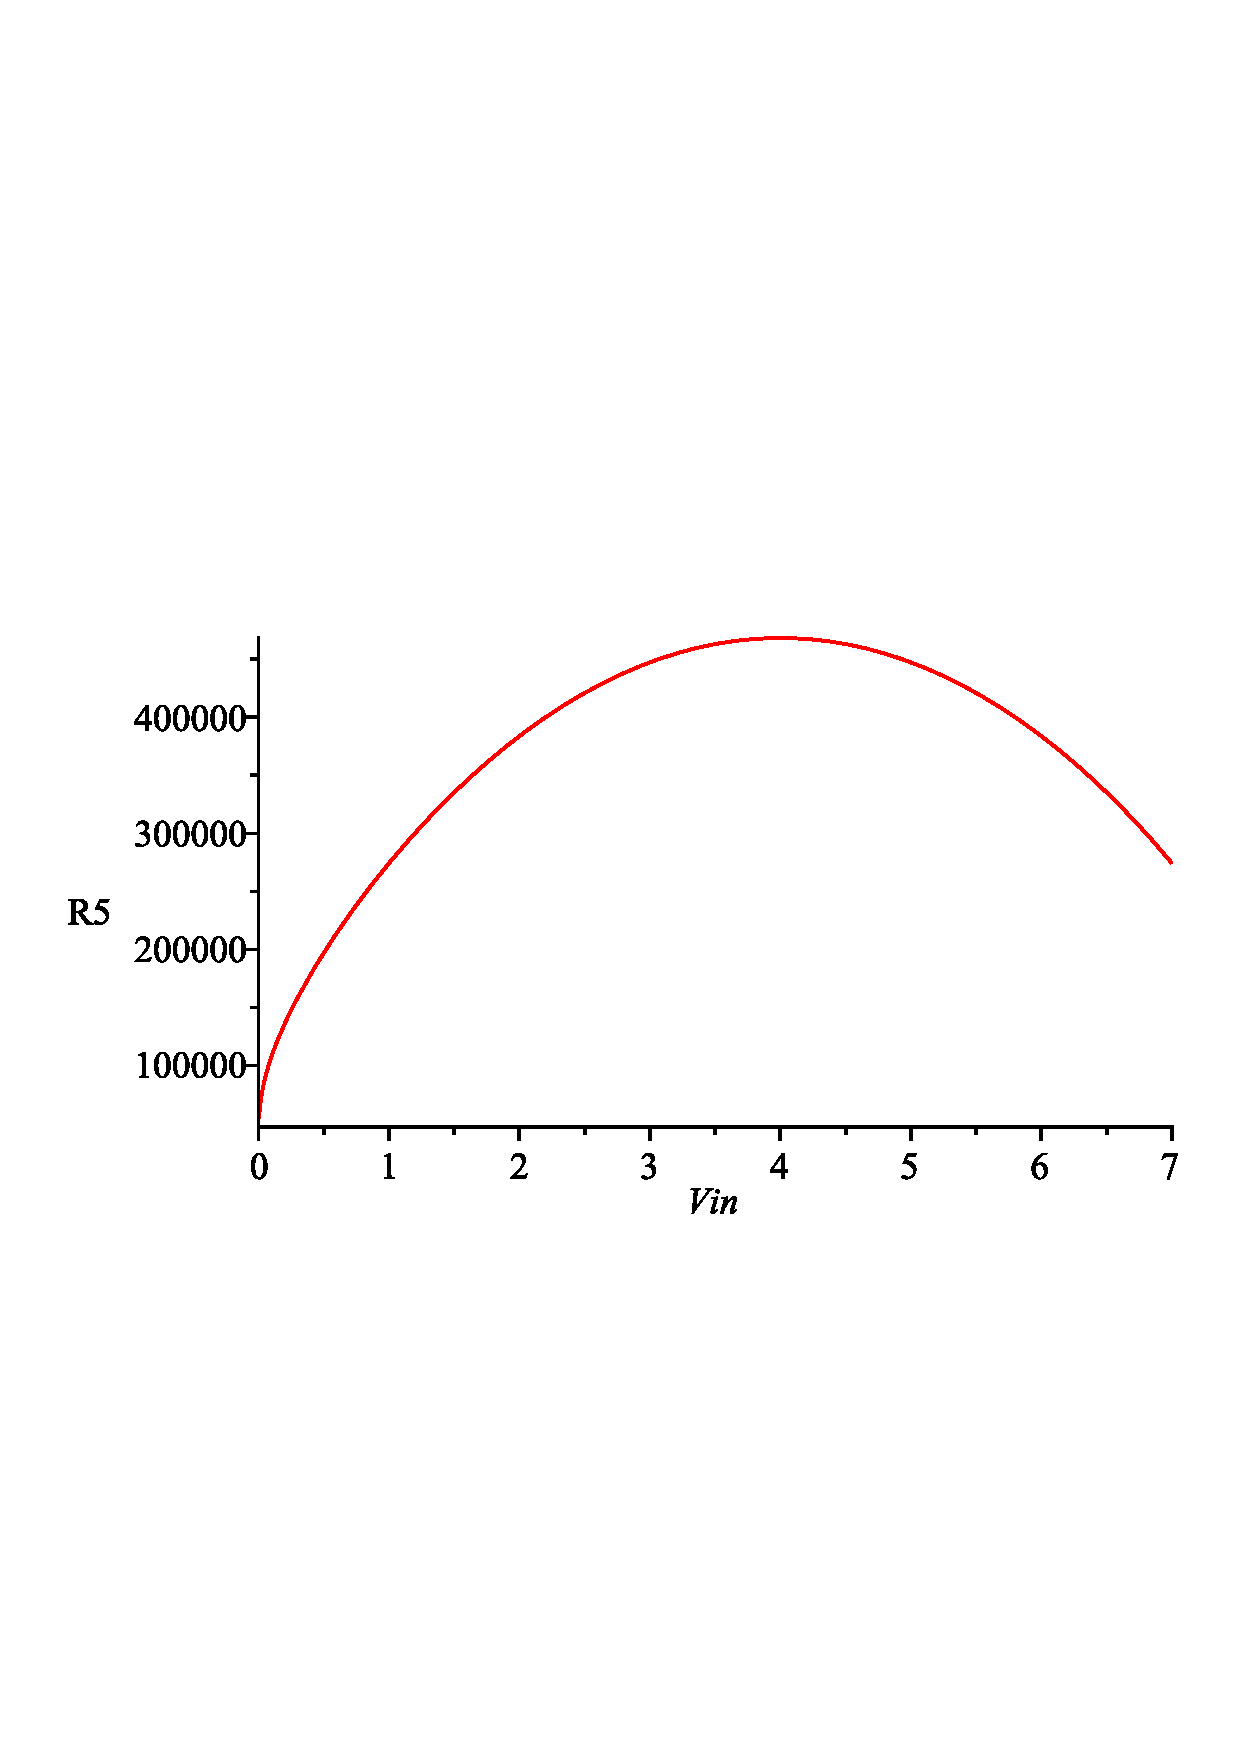
\includegraphics[width=.70\textwidth]{images/VinR5.pdf}
    \caption{Input Voltage Vs Desired Value for $R_5$ for 300 Hz Frequency}
\end{figure}

A circuit simulation confirms a nominal frequency very close to 300 Hz.
To verify the frequency, a Fourier transform of the oscillator output for $V_{in} = 2.28 V$ and $R_5 = 406.1 k\Omega$ is shown in figure 3. 
It can be seen that the dominant frequency is approximately 300 Hz.
%	TODO: Why approximately
A theoretical plot of duty cycle over a range of input voltages may be seen in figure 4.

\begin{figure}[h]
    \label{fig:FFT}
    \centering
    \includegraphics[width=.70\textwidth,bb=0 0 1056 406]{images/FFT.png}
    \caption{Fast Fourier Transform of Simulated Oscillator Output}
\end{figure}

\begin{figure}[h]
    \label{fig:dutycycle}
    \centering
    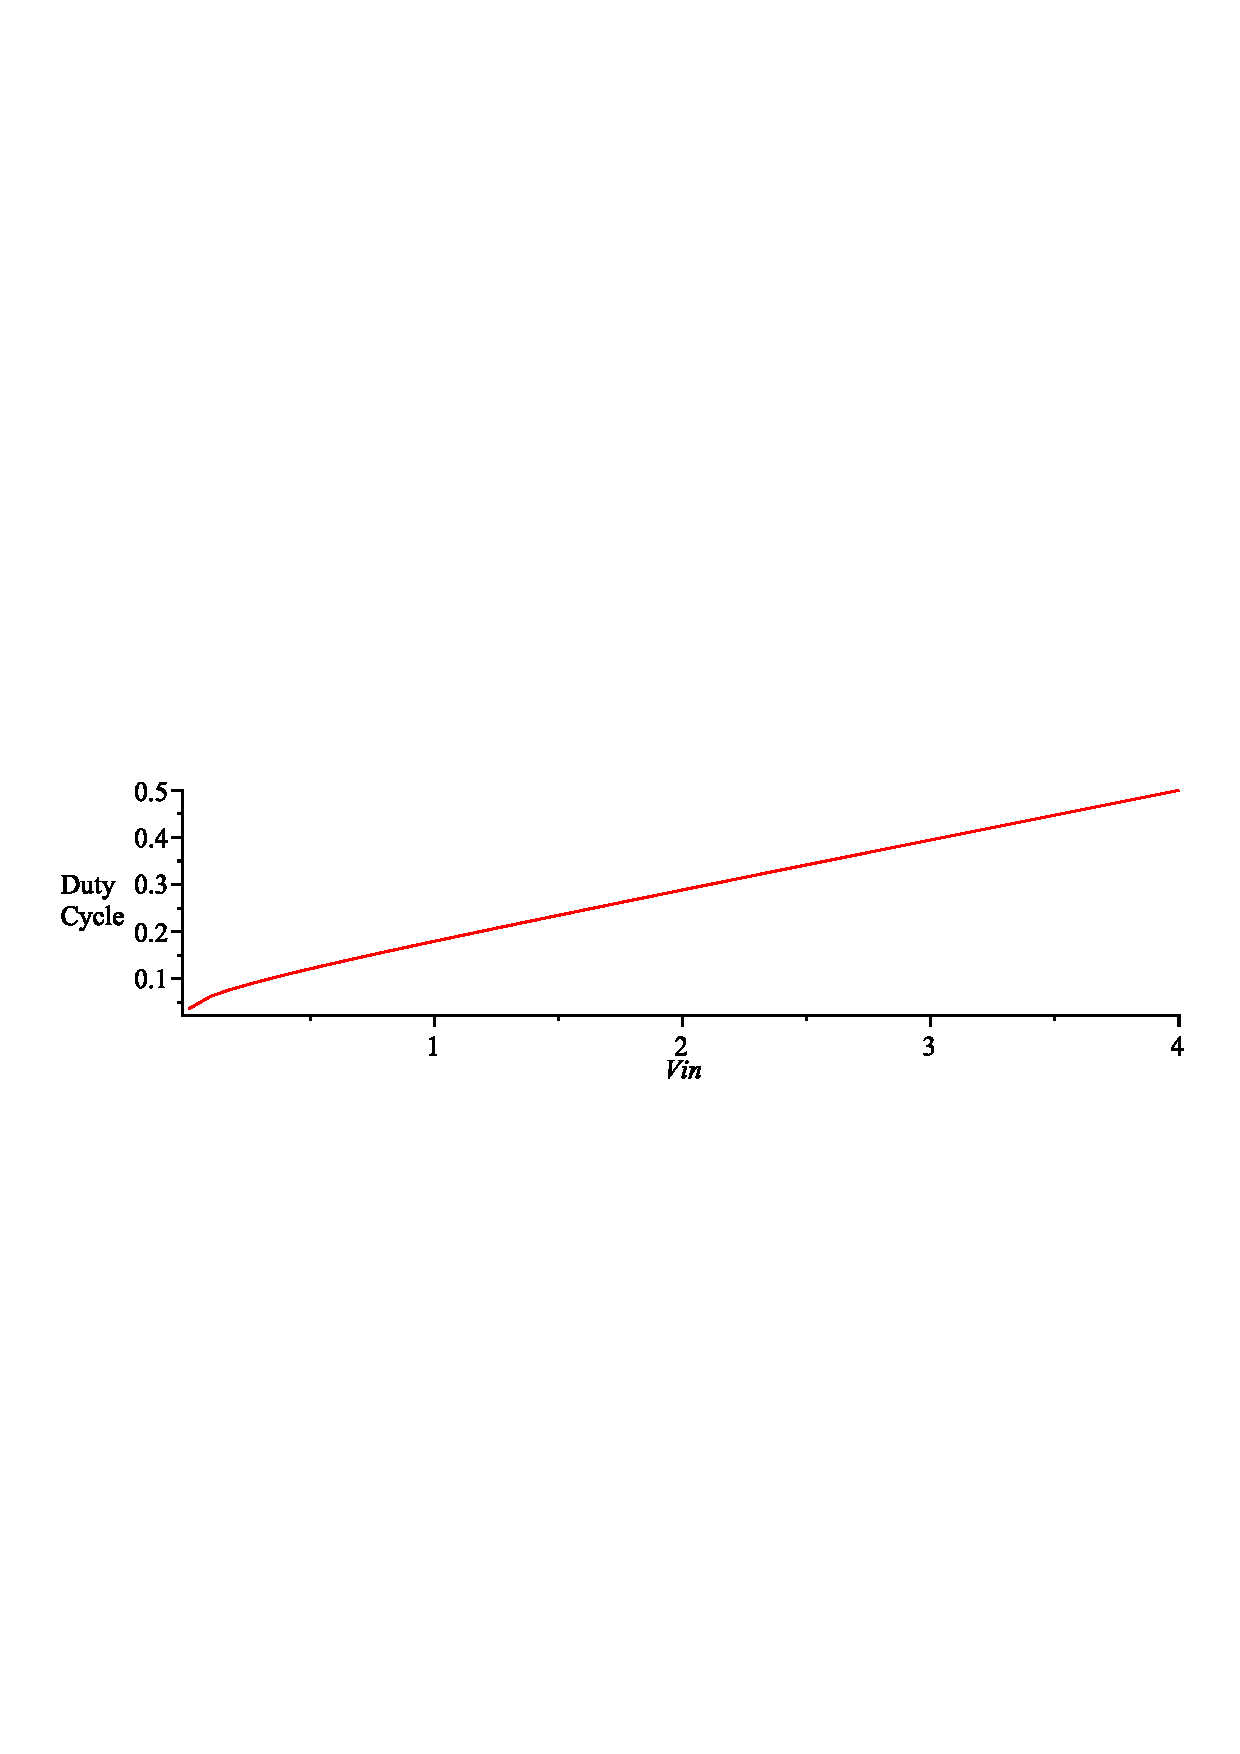
\includegraphics[width=.70\textwidth]{images/dutycycle.pdf}
    \caption{Oscillator Duty Cycle for $V_{in} = 0$ to $V_{in} = {\frac {V^+}{2}}$}
\end{figure}

\subsection{Input Output Characterization}

The input-output characteristics of the amplifier were examined for the simulated circuit and the actual circuit.
The result may be seen in figure 5.
It should be noted that the simulated circuit had no load whereas the actual circuit was driving the motor, with no load.
Sample values are given in table \ref{tbl:iovalues}.
Refer to section \ref{sec:tf} for an overview of the process used to obtain experimental values.

\begin{figure}[h]
    \label{fig:io}
    \centering
    \includegraphics[width=.70\textwidth,bb=0 0 1149 467]{images/OutputVoltage.png}
    \caption{Input-Output Characterization for Simulated (Unloaded) and Actual (Loaded with Motor) Circuit}
\end{figure}

\begin{table}[h]
	\centering
	\caption{Input-Output Characterization}
	\label{tbl:iovalues}
	\vspace{6pt}
	\footnotesize
	\begin{tabular}{ccc}
		\toprule
		$V_{in}$ & $V_{out}$ (Actual) & $V_{out}$ (Simulated) \\
		\midrule
		3.8 & 8.06 & 6.4819629 \\
		2.90 &7.8 & 2.1355862 \\
		2.799 &7.71 & 1.6661552 \\
		2.6 &7.38 & 0.7739846 \\
		2.515 &7.0 & 0.394138 \\
		2.459 &6.70 & 0.1553944 \\
		2.43 &6.48 & 0.0338252 \\
		2.4 &6.0 & 0.0016906 \\
		2.39 &5.95 & 0.0012864 \\
		2.34 &4.89 & 0.0002554 \\
		2.31 &3.77 & -0.0002944 \\
		2.29 &2.8 & -0.0008018 \\
		2.28 &2.72 & -0.001161 \\
		2.27 &1.23 & -0.001596 \\
		2.265 &1.2 & -0.0018552 \\
		2.261 &1.1 & 0.8382106 \\
		2.25 &0.81 & -0.0029108 \\
		1.81 &-1.9 & -1.7913446 \\
		1.791 &-2.75 & -1.8549068 \\
		1.752 &-4.56 & -2.1259024 \\
		1.746 &-4.92 & -2.0894574 \\
		1.709 &-5.96 & -2.2841442 \\
		1.665 &-6.64 &- 2.5689882 \\
		1.630 &-6.94 & -2.748412 \\
		1.572 &-7.27 & -3.0502118 \\
		1.555 &-7.33 & -3.1671898 \\
		1.425 &-7.64 & -3.82 \\
		0.338 &-8.04 & -7.00 \\
		\bottomrule
	\end{tabular}
\end{table}


%
%Section: Verification and Test
%	- 
%
% Gain characteristics
% 	- Transfer function
% 	- Data plots
% 	- How we got them (testing process)
% 	
%
% Heat sink and power dissipation
% 	- Based on measured power draw
% 	- How we got them (testing process)
% 	
\section{Verification and Testing}

This section details lab activities to test and verify the circuit. 
After the provided circuit components were soldered to the PCB, two tests were performed.
The first found the experimental transfer function between amplifer input voltage and voltage output to the motors.
The second test estimated the power dissipated by the MOSFET transistors.

\subsection{Amplifier Transfer Function}
\label{sec:tf}

To obtain the response of the motor to an applied input, the input voltage to the amplifier was adjusted using a potentiometer, 
Multimeters were used to capture to between the potentiometer output and ground (the amplifier input voltage input) and the associated voltage drop across the motor (output voltage).
During testing, an unloaded motor was connected to the amplifier.
By taking roughly thirty measurements for input voltages in the range of 0 to 4V, it was possible to establish the experimental relationship seen in figure 5, for a given circuit input voltage of 8V.

%TODO: Why so different

\subsection{Heat Sink Design}

Given the high-power nature of the MOSFET drive transistors, it is important to ensure they do not exceed their maximum operating temperature.
To this end, the maximum thermal resistance factor, $\theta_{JA}$ for which the MOSFETs may operate safely was calculated.
The thermal resistance factor is given by equation \ref{eq:theta}.

\begin{equation}
	\label{eq:theta}
	\theta_{JA} = {\frac{T_J - T_A} {P_D}}
\end{equation}

In this equation $T_A$ represents the ambient temperature, for which $25^{\circ}C$ was used. 
The $T_J$ value, or maximum silicon junction temperature, is supplied by the manufacturer and was seen to be $175^{\circ}C$ for both types of transistors.
% TODO: reference datasheet
The $P_D$ value is the power dissipated and is calculated by subtracting the power measured at the load from the power measured at the supply.
To determine the load power, two multimeters were used to measure voltage drop across the motor and current through the motor. 
During the test, the motor was loaded by attempting to hold the shaft.
The supply power was similarly calculated by measuring input voltage and current to the entire circuit.
It was assumed that that the power dissipation for components other than the MOSFETs was negligible.
For a loaded motor, it was seen that, Input: 10v @ 0.65 A, Output: 8.25v @ 0.70 A, producing the $P_D$ value in equation \ref{eq:PD} . 

\begin{equation}
	\label{eq:PD}
	P_D =  P_S - P_L = \left({10 V}{\times}{.65 A}) - ({8.25 V}{\times}{.70 A}\right)
	    { = 0.725 W }
\end{equation}

Based on the experimentally observed power dissipation, the maximum thermal junction resistance may be calculated.
This is shown in equation \ref{eq:theta2}, assuming all power is dissipated by a single MOSFET.
It should be noted that due to the H-bridge design, power dissipation is actually split across two different transistors.
The Junction-to-Ambient thermal resistance for both MOSFET transistors is less than  $63^{\circ}C/W$.
As such, it is clear that based on experimentally observed power dissipation, there is no need for a heat sink.

\begin{equation}
	\label{eq:theta2}
	\theta_{JA_{MAX}} = \left({175 - 25}\right) {0.725 }
	{ = 206  ^{\circ}C/W}
\end{equation}


% Conclusion
% 	- John
\section{Conclusion}
\label{sec:Conclusion}

This report has discussed the basic features of the controller design such as filters, signal conditioning, software PWM, and voltage control. 
Furthermore, the report explained the approach taken to design the controller to maximize performance. 
Limitations to simulating this specific controller were discussed in addition to general system and controller limitations including proposed solutions to improve the response and increase the execution time. 
Finally the final system performance was presented, an overall time of 0.7432 seconds based on the common method used for measuring.


%#######################################
%	References
%#######################################

%\cleardoublepage

%\bibliography{References}
%\addcontentsline{toc}{chapter}{\hspace{13pt}References}

%#######################################
%	Appendix
%#######################################

%\begin{appendix}
%\onecolumn
%\section{Controller Code}

asdf

asdf
%\end{appendix}

\end{document}